\chapter*{Un jugador de baseball}
\section*{Un jugador de baseball}
    Un jugador de baseball batea la pelota a 3 ft de altura sobre el plato en dirección a la barda del jardín central que está a 400 ft de distancia de home y tiene 10 ft de altura. La pelota sale con rapidez de 115 $\frac{ft}{s}$ y un ángulo de elevación de 50° sobre la horizontal.
    
    1) Sabemos que el vector de movimiento $\vec{v}=115\frac{ft}{s}$ de la pelota se puede descomponer en dos direcciones de velocidad, movimiento rectilíneo y tiro vertical y caída libre ya que su comportamiento es en dos grados de libertad $$r:\left[0,t\right]\rightarrow \mathbb{R}^2_{(x,y)}$$
    $\therefore$ la componente horizontal del  vector de la bola está representada por la formula del mov. rect. uniforme.$x(t)=v_x(t)=v_{0_x}\Rightarrow x(t)-x_{0}=v_{0_x}(t)\therefore x(t)=v_{0_x}(t)$
    Como el movimiento no es recto completamente, si no que tiene un ángulo de inclinación, requerimos del coseno para calcular la fracción de la velocidad que le corresponde. $$\vec{\|vx\|}=\vec{\|v\|}cos\;\theta = 115cos\;50 = 73.91\frac{ft}{s}$$
    2) La componente vertical del vector resultante está representada por la caída libre, la cual denotamos como $v(t)=gt$.
    El área bajo la recta de velocidad respecto al tiempo representa el desplazamiento del objeto $$\therefore y(t)-y(0)=\frac{1}{2}gt^2$$
    como el movimiento de caída crece un lapso de tiempo y luego decrece hasta tocar el suelo nuestra aceleración es negativa y, además, consideremos que el movimiento empieza a una distancia distinta de cero.$$y(t)-y(0)=v_{0_y}t-\frac{1}{2}gt^2$$ tomando en cuenta que la gravedad es de $32\frac{ft}{s^2}$ $$\Rightarrow y(t)=y(0)+v_{0_y}t-\frac{1}{2}gt^2$$ donde $v_{0_y}$ representa la velocidad respecto de la componente en y, $$\therefore \vec{\|v_y\|}=115 sen\theta 50=89.09\frac{ft}{s}$$, sustituyendo tenemos$$y(t)=3+89.09\frac{ft}{s}t-16t^2$$ donde 3 es la altura en pies donde el bat impacta con la pelota.
    
    \vspace{5mm} %5mm vertical space        
    
    3) Sabemos que $x(t)$ es la fórmula de la distancia que tomará la bola respecto a cada segundo que dura el movimiento. Queremos averiguar cual sería el tiempo en el que la pelota está a 400 metros del bateador para poder determinar si la pelota sobrepasa la barrera
    $$x(t)=73.91\frac{ft}{s}t=400ft\therefore t=\frac{400ft}{73.91\frac{ft}{s}}=5.4119s$$
    La pelota tarda $5.4119s$ en llegar a los $400 ft$ de distancia.
    Ahora, para saber la posición de la pelota en ese tiempo tenemos que sustituir el valor del tiempo en la fórmula que nos dice a que altura llega la bola respecto a su desplazamiento.
    $$y(5.4119)=3+89.09\frac{ft}{s}(5.4119s)-16(5.4119s)^2$$
        $$y(5.4119) \simeq 11.1156ft$$
    Concluimos que la pelota supera la barrera de $10ft$ de altura que está a $400 ft$ de distancia ya que la pelota en ese mismo instante se encuentra a una altura superior que el de la barrera.
    
    \vspace{5mm} %5mm vertical space        
    
    Consideremos que la bola choca con un obstáculo a $5ft$ de altura después de pasar la barrera, lo primero que queremos saber es cuando $y(t)=5$
    \begin{gather*}
        y(t)=5=y(t)=3+89.09\frac{ft}{s}t-16t^2\\
        2=88.0951t-16t^2\\
        t=(88.0951-16t)t\\
        t_1=2\\
        t_2:(88.0951-16t_2)=2\\
        -16t_2=-86.0951\\
        t_2=\frac{-86.0951}{-16}\\
        t_2=5.4839s
    \end{gather*}
    Tengamos en cuenta el movimiento parabólico que tiene la pelota, entonces pasa en 2 tiempos diferentes a los $5 fts$, considerando el mayor de ellos (parte final del movimiento), tenemos que, para saber la posición a la que se encontraba la bola en ese tiempo usaremos la formula de posición $x(t)$.
    \begin{gather*}
        x(t)=73.9206t\\
        x(5.4839)=73.9206\frac{ft}{s}(5.4839s)\\
        x(5.4839)\simeq405.314ft
    \end{gather*}
    $\therefore$ Concluimos que el movimiento termina, o por lo menos no está definido después de $5.4839s$ en la distancia max. de $405.314ft$.
    
    \vspace{5mm} %5mm vertical space        
    
    c) Para calcular el valor máximo de altura a la que se encuentra la bola en el movimiento tenemos que hacer uso de la primer derivada de la fórmula $y(t)$ que representa la posición de altura para cada valor del tiempo.
    \begin{gather*}
        y'(t)=88.0951t-32t\\
        y'(t)=0=88.0951t-32t\\
        -32t=-88.0951\\
        t=\frac{-88.0951}{-32}\\
        t\simeq 2.7529s
    \end{gather*}
    $t\simeq 2.7529s$ es el valor aproximado del tiempo en el que se encuentra a la altura máxima, este valor lo sustituimos en la ecuación $y(t)$ para saber cual es la posición en ese tiempo.
    \begin{gather*}
        y(2.7529s)=3+89.09\frac{ft}{s}(2.7529s)-16(2.7529s)^2
        y(2.7529s)\simeq 124.2617ft
    \end{gather*}

    \begin{center}
        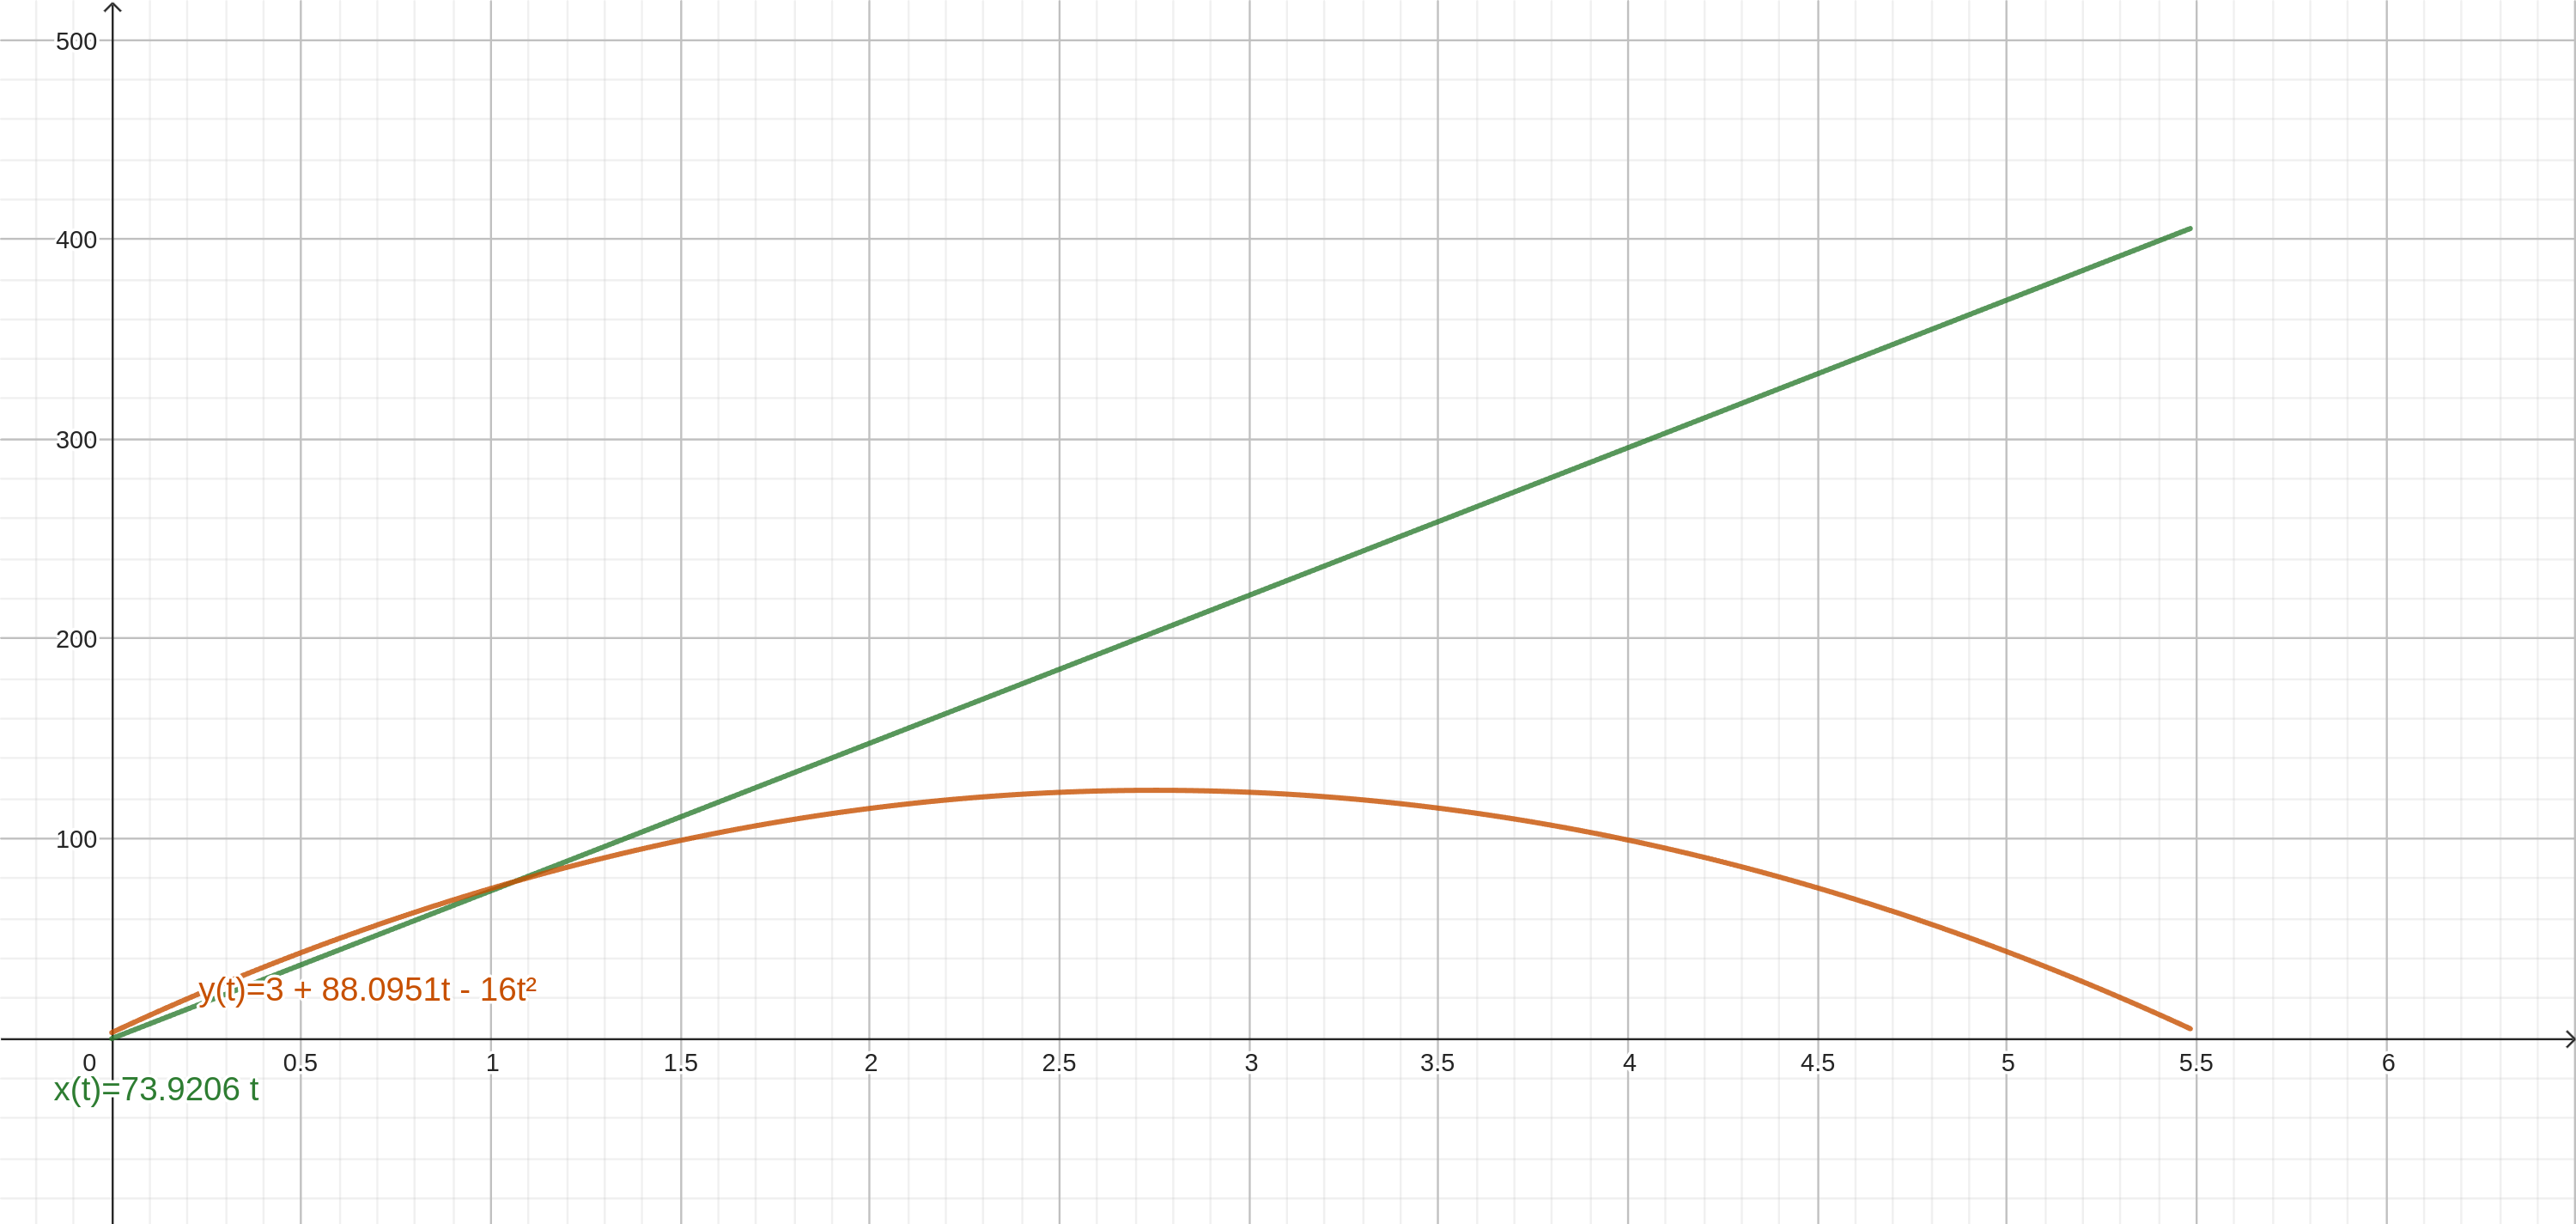
\includegraphics[height = 0.3\textheight]{recursos/geogebra-export(1).png}\par
    \end{center}
    Trayectoria    
    \begin{center}
        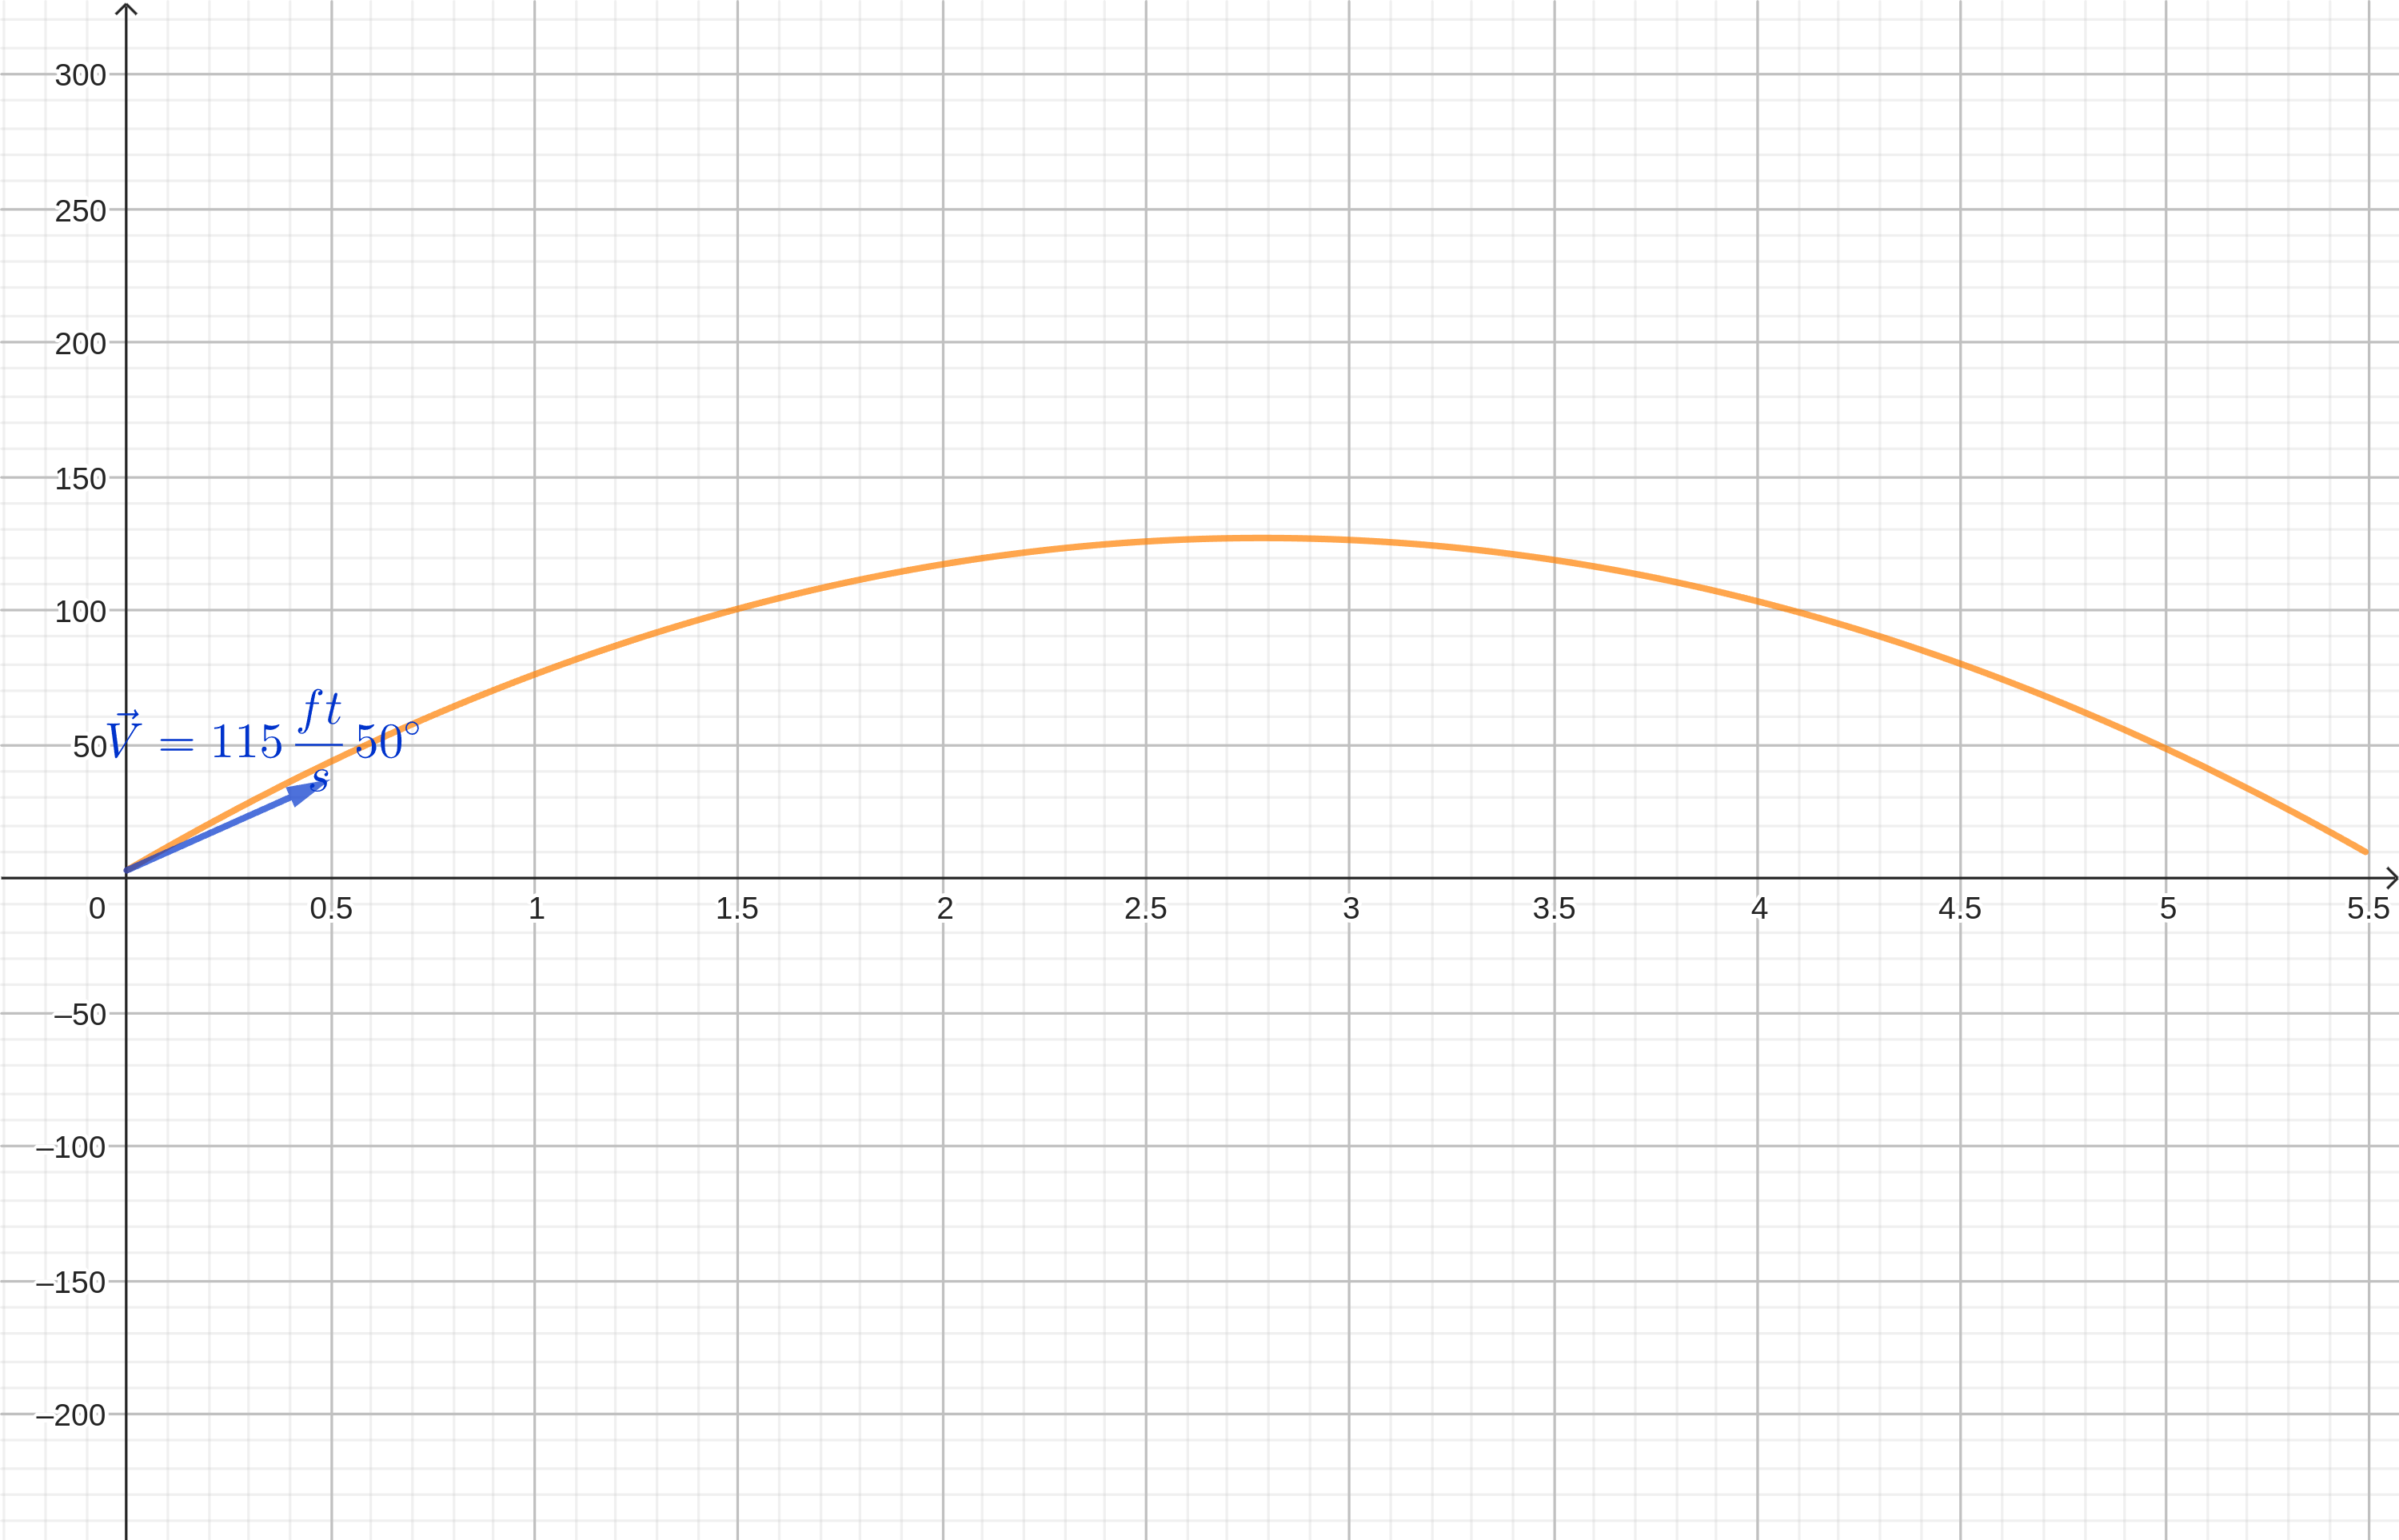
\includegraphics[height = 0.3\textheight]{recursos/geogebra-export(2).png}\par
    \end{center}
